\label{game}

In this chapter we want to have the contribution of the human intelligence in making decisions, so we made a simulation game using \textit{Unity}.

%===============================================================================

\section{Introduction to Unity}

Unity is a cross-platform game engine (Fig. \ref{UnityInterface}) developed by Unity Technologies and used to develop video games for PC, consoles, mobile devices and websites. It is a free software (https://unity3d.com/),working with C\# programming language. 
 

\begin{figure}[H]
	\centering
	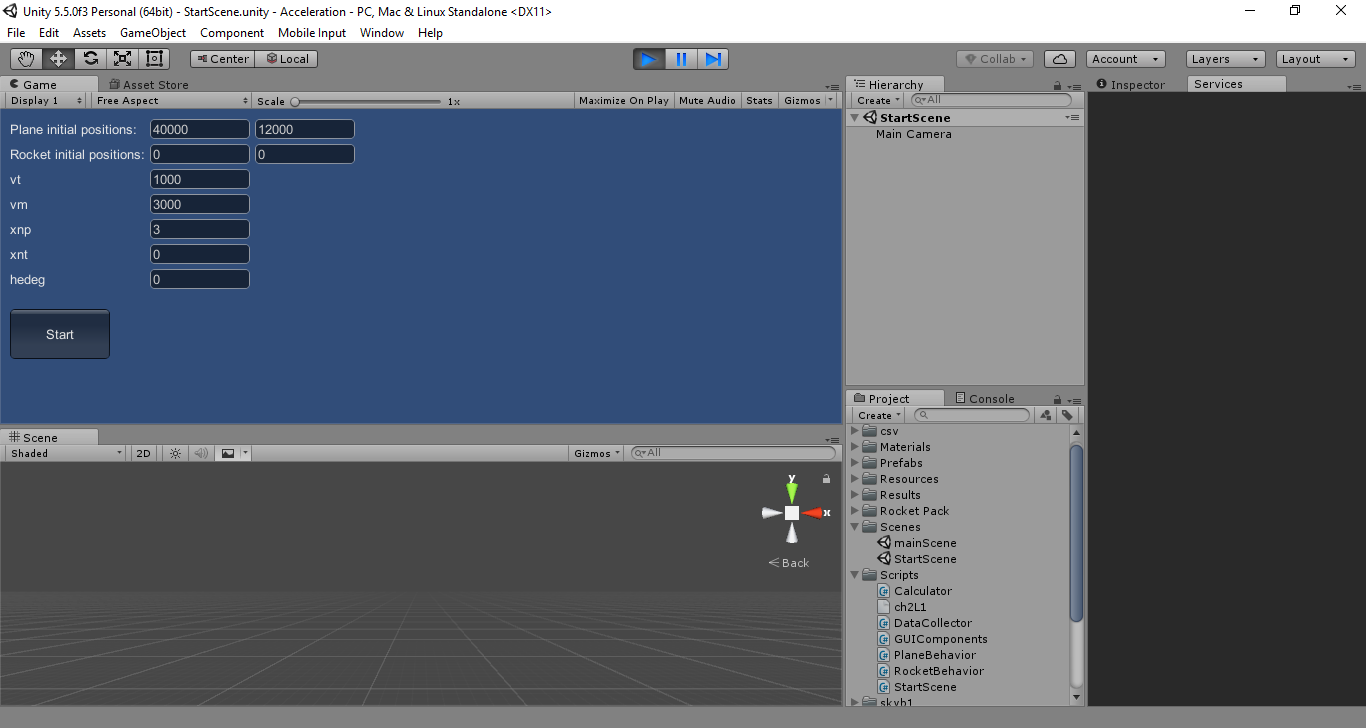
\includegraphics[scale = 0.35]{fig/unityInterface.PNG}
	\caption{Unity game engine interface }
	\label{UnityInterface}
\end{figure}

%===================================================================================

\section{Methodology of the game}

The game (Fig. \ref{UnityGame}) consists of two objects: plane (Target) and missile (Attacker). A human player controls the increasing and decreasing of the target acceleration (XNT) by two arrows on the keyboard. The missile object is moving on according to the proportional navigation guidance law (in sec. \ref{PNeq}).
 
 \begin{figure}[H]
 	\centering
 	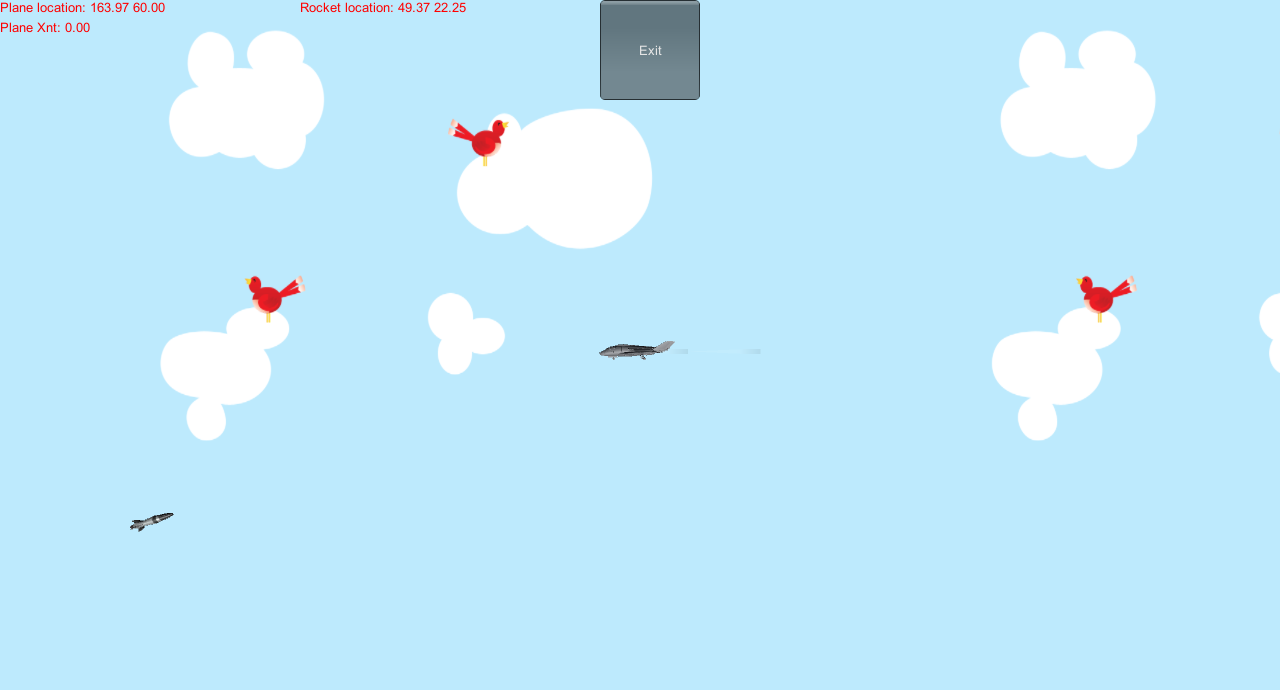
\includegraphics[scale = 0.35]{fig/unityGame.PNG}
 	\caption{Unity game for simulating Target-Attacker engagement}
 	\label{UnityGame}
 \end{figure}
 

Each game consists of two scenes:

\begin{enumerate}
	\item Starting scene.
	\item Game scene, which updated each frame per second.
\end{enumerate}

In the starting scene there is data fields (position, velocity, ...). After this scene ends, all the data are destroyed, so we save the information we need in file called "player prefs".

The game scene consists of some objects, each object has his own script, this script must contain 2 points:
\begin{itemize}
	\item Start: initialization.
	\item Updated : every frame.
\end{itemize} 

In our game we have 3 objects:
\begin{enumerate}
	\item \textbf{Plane:} its script contain some commands to control the plane with two arrows in the keyboard, which increase and decrease the target acceleration by upward arrow and downward arrow respectively. 
	\item \textbf{Missile:} it does not contain a script, the equations controlling its behavior is in the script with the "Data collector" object.
	\item \textbf{Object "Data collector":} its script consists of:
	
	\begin{itemize}
		\item Start
		\begin{enumerate}
			\item initialization of the variables in the equations.
			\item set the location of all objects (plane and missile).
		\end{enumerate}
		\item Update 
		\begin{enumerate}
			\item get plane location.
			\item execute your equations.
			\item update rocket location (according to PN equations).
			\item update informations to be printed to excel.
			\item check the breaking condition, if true, load starting scene.
		\end{enumerate}
	\end{itemize}


\end{enumerate} 




%===================================================================================
 
\section{Results}

